\documentclass[12pt]{article}

\usepackage{graphicx}

\graphicspath{ {/} }


\pagestyle{empty}
\setcounter{secnumdepth}{2}

\topmargin=0cm
\oddsidemargin=0cm
\textheight=22.0cm
\textwidth=16cm
\parindent=0cm
\parskip=0.15cm
\topskip=0truecm
\raggedbottom
\abovedisplayskip=3mm
\belowdisplayskip=3mm
\abovedisplayshortskip=0mm
\belowdisplayshortskip=2mm
\normalbaselineskip=12pt
\normalbaselines

\begin{document}

\vspace*{0.5in}
\centerline{\bf\Large Design Document}

\vspace*{0.5in}
\centerline{\bf\Large Team PB-PK}

\vspace*{0.5in}
\centerline{\bf\Large 18 March 2018}

\vspace*{1.5in}
\begin{table}[htbp]
\begin{center}
\begin{tabular}{|l | c|}
\hline
Name & ID Number \\
\hline\hline
Noemi Lemonnier & 40001085 \\ \hline 
Genevieve Plante-Brisebois & 40003112 \\ \hline 
Han Gao & 40053734 \\ \hline 
Theo Grimond & 27276044 \\ \hline 
Real Nguyen & 27566263 \\ \hline 
Ornela Bregu & 26898580 \\ \hline 
William Prioriello & 27080956 \\ \hline 
Tiantian Ji & 27781083 \\ \hline 
Dong-Son Nguyen-Huu & 40014054  \\ \hline 
Ashesh Patel & 40018519 \\ \hline 
Sabrina Rieck & 40032864 \\ \hline
\hline
\end{tabular}
\end{center}
\caption{Team}
\end{table}

\clearpage

\section{Introduction}

The introduction of the document provides an overview of the entire document,
briefly introducing what are its goals, and what information is to be found in it.

\section{Architectural Design} \label{sec:arch}

This section must give a high-level description of the system in terms of its modules
and their respective purpose and exact interfaces.

\subsection{Architectural Diagram}

A UML class diagram or package diagram depicting the high-level structure of the system,
accompanied by a one-paragraph text describing the rationale of this design.
It is mandatory that the system be divided into at least two subsystems,
and that the purpose of each of these subsystems be exposed here.

\subsection{Subsystem Interface Specifications}

Specification of the software interfaces between the subsystems,
i.e. specific messages (or function calls) that are exchanged by the subsystems.
These are also often called ``Module Interface Specifications''.
Description of the parameters to be passed into these function calls in order to have a service fulfilled,
including valid and invalid ranges of values.
Each subsystem interface must be presented in a separate subsection.

\section{Detailed Design} \label{sec:detail}

Complete description of the system design, describing one subsystem separately in respective subsection.
UML class diagrams are to be used, as well as a short textual description describing the purpose of each class.





\subsubsection{Detailed Design Diagram}

UML class diagram depicting the internal structure of the subsystem,
accompanied by a paragraph of text describing the rationale of this design.
\subsection{Cash Spending Class}
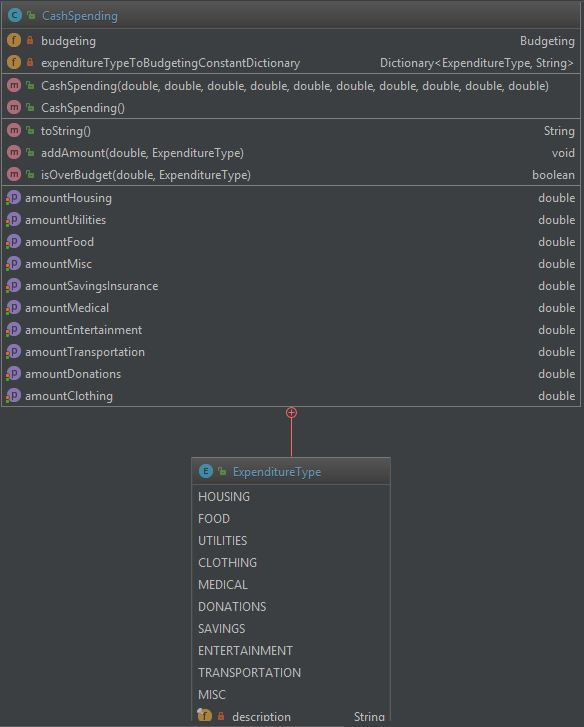
\includegraphics{cashspending}

\caption{Cash Spending Class Diagram}

\subsubsection{Units Description}
List each class in this subsystem and write a short description of its purpose,
as well as notes or reminders useful for the programmers who will implement them.
List all attributes and functions of the class.

\begin{center}
\begin{tabular}{|p{2cm}||p{15cm}|}
\hline
Class name & CashSpending \\
\hline
Description & Contains basic business logic that manipulates the user's spending data model\\
\hline

Attributes & budgeting,
expenditureTypeToBudgetingConstantDictionary, 
amountHousing,
amountUtilities,
amountFood,
amountMisc,
amountSavingsInsurance,
amountMedical,
amountEntertainment,
amountTransportation,
amountDonations,
amountClothing\\
\hline
Methods & CashSpending(),
toString(),
addAmount(double, ExpenditureType),
isOverBudget(double, ExpenditureType)\\
\hline
\end{tabular}
\end{center}


\section{Dynamic Design Scenarios}

Describe some (at least two) important execution scenarios of the system using UML sequence diagrams.
These scenarios must demonstrate how the various subsystems and units are interacting to achieve a system-level service.
Units and subsystems depicted here must be compatible with the descriptions provided in
section \ref{sec:arch} and \ref{sec:detail}.

\end{document}
